
\documentclass[10pt]{beamer}
\usepackage{amsfonts}
\usepackage{amssymb}
\usepackage{amsmath}
\usepackage{bm}
\usepackage{pgffor}
\usepackage{microtype}
\usepackage{graphicx}
\graphicspath{ {./pic/} }

\long\def\comment#1\endcomment{}


\usetheme{Singapore}
\usecolortheme[rgb={1,.1,.1}]{structure}
%carini NavyBlue RoyalBlue JungleGreen
%\usecolortheme{sidebartab}
\usefonttheme[]{structurebold}
\useinnertheme[shadow]{rounded}
%\useoutertheme[left]{sidebar}
\useinnertheme[shadow]{rounded}
%\setbeamertemplate{items}[ball unnumbered]
\setbeamersize{text margin left=.9cm,
			   text margin right=.9cm} 




\theoremstyle{definition}
\newtheorem{definizione}{Definizione}
\theoremstyle{plain}
\newtheorem{teorema}{Teorema}
%\newtheorem{lemma}{Lemma}

\setbeamertemplate{navigation symbols}{}
%\mode<presentation>


\def\R{\mathbb R}
\def\Cal#1{{\cal #1}}
\def\form#1#2{(\,#1\,,\,#2\,)}
\def\bform#1#2{\bigl(\,#1\,,\,#2\,\bigr)}
\def\Bform#1#2{\biggl(\,#1\,,\,#2\,\biggr)}
\def\norm#1{\Vert #1\Vert}
\def\bnorm#1{\bigl\Vert #1\bigr\Vert}
\def\Bnorm#1{\biggl\Vert #1\biggr\Vert}
\def\opnorm#1{|\mskip-1.5mu|\mskip-1.5mu|#1|\mskip-1.5mu|\mskip-1.5mu|}
\def\hbyw#1#2{\vbox to #1{\vfil \hbox to #2{\hfil}}}
\def\hbywtop#1#2{\vtop to #1{\vfil \hbox to #2{\hfil}}}
\def\lK{{\lower.5ex\hbox{$\scriptstyle K$}}}
\def\lX{{\!\!\lower.5ex\hbox{$\scriptstyle X$}}}
\def\lXf{{\lower.5ex\hbox{$\scriptstyle X, f$}}}
\def\lXyf{{\lower.5ex\hbox{$\scriptstyle X\cup\{y\}, f$}}}

\def\line#1{\hbox to\hsize{#1}}


%%%%%%%%%%%%%%%%%%%%%%%%%%%%%%%%%%%%%%%


\title{ON THE PROBLEM OF RECOVERING\\
	  DISCONTINUOUS FUNCTIONS\\
	  FROM SCATTERED DATA}
\author{Matteo Caoduro}
\date{18 marzo 2021}
%\institute{\normalsize \emph{Relatore:} Prof.ssa\, Milvia Francesca Rossini}



\begin{document}

\begin{frame}
  \titlepage
\end{frame}



\part<presentation>{Main Talk}

\section{Introduzione}


\begin{frame}
\null\vskip.1cm
\line{\kern-.3cm\vbox{\hbox{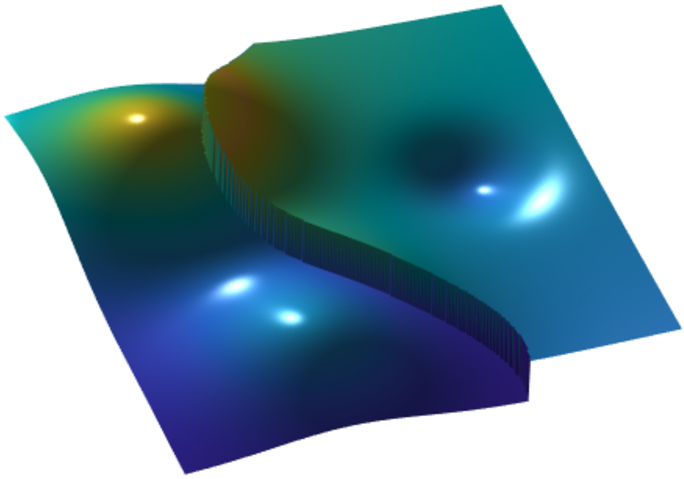
\includegraphics[width=.5\hsize]{f1intro_ori.pdf}}\vfil
\hbox{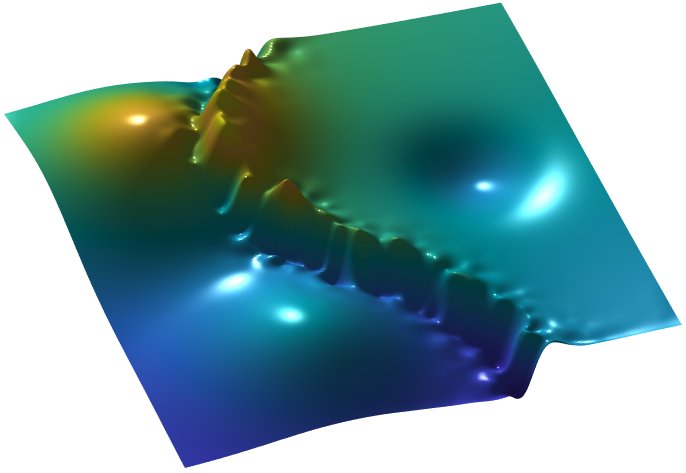
\includegraphics[width=.5\hsize]{f1intro_rec.pdf}}}
\hfil\raise1cm\hbox{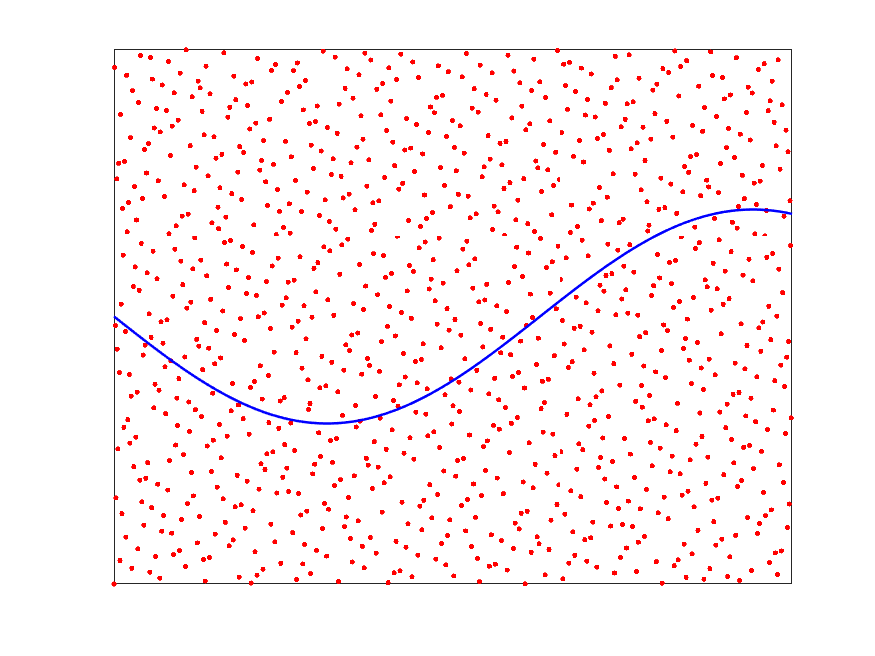
\includegraphics[width=.5\hsize]{f1intro_datasites.pdf}}\kern-.3cm}
\end{frame}


\begin{frame}
\frametitle{Obiettivo}
Ricostruire  una \alert{funzione discontinua}~$f:\Omega\to\R$, con $\Omega\subset\R^2$, conoscendo i valori $F = f(X) = \{f_1,f_2,\dots f_N\}$ che essa assume su un insieme di \alert{dati sparsi} $X=\{x_1,x_2,\dots,x_N\}\subset\Omega$

\begin{itemize}
\item evitando il fenomeno di Gibbs,
\item riproducendo fedelmente $f$ in prossimità delle curve di discontinuità.
\end{itemize}

\bigskip\medskip

\alert{Ipotesi}: $f$ regolare (almeno continua) su sottoinsiemi~$\Omega_j$ disgiunti tali che $\Omega = \cup_j \Omega_j$, e discontinua lungo $\partial \Omega_j$.

\medskip
Non si hanno informazioni sui sottoinsiemi $\Omega_j$ né sulle curve di discontinuità.



\end{frame}

\begin{frame}
%Per ricostruire correttamente la funzione è necessario determinare i sottoinsiemi~$\Omega_j$.
%La funzione poi viene ricostruita su ciascun sottoinsieme separatamente.

%\medskip
Tre fasi:

\bigskip\smallskip

\begin{itemize}
\item Raggruppare  $X$ in sottoinsiemi $X_j$ tali che $X_j\subset \Omega_j$:
	 si utilizza un \alert{classificatore} di regolarità basato su interpolanti con basi radiali per analizzare localmente in $\Omega$ i dati $(X,f(X))$;

\bigskip\smallskip

\item Ricostruire i sottoinsiemi $\Omega_j$  mediante {\em Support Vector Machines};

\bigskip\smallskip

\item Interpolare $(X_j, f(X_j))$ su $\Omega_j$ usando basi radiali.
\end{itemize}
\end{frame}



\begin{frame}
\frametitle{Kernel e spazi nativi}
\begin{itemize}
\item
Ogni \alert{kernel}~$K:\Omega\times\Omega\to\R$ simmetrico e definito positivo, con $\Omega\subseteq\R^d$, genera uno spazio di Hilbert~$\Cal N_K$, il suo \alert{spazio nativo}:
$$
\Cal N_K = \overline{\operatorname{span}\{K(\cdot, y):\> y\in\Omega\}\hbyw{2ex}{0em}},
$$
con prodotto scalare
$$
\Bform{\sum_{j=1}^N\alpha_jK(\cdot, x_j)}{\sum_{k=1}^M\beta_k K(\cdot,y_k)}_{\!\!K} =  \sum_{j=1}^N\sum_{k=1}^M \alpha_j \beta_k K(x_j,y_k).
$$


\item
$K$ è \emph{riproducente} in $\Cal N_K$:
\begin{itemize}
\item $K(\cdot, y) \in\Cal N_K$, \quad per ogni $y\in\Omega$,
\item  $\form{K(\cdot, y)}f_{\lK} = f(y)$,\quad per ogni $f\in\Cal N_K$, $y\in\Omega$.
\end{itemize}
\end{itemize}
\end{frame}


\begin{frame}
\frametitle{Interpolazione in $\Cal N_K$}
\begin{itemize}
\item 
In $\Cal N_K$ il problema dell’interpolazione ha sempre soluzione.  Infatti la matrice $\bm A$ con elementi
$$
A_{i,j} = K(x_i, x_j), \qquad  X=\{x_1,x_2,\dots,x_N\}
$$
è definita positiva.

\item
La funzione $s_\lXf = \sum_{j=1}^N \alpha_j K(\cdot, x_j)\in\Cal N_K$, ottenuta risolvendo il sistema lineare
 $$
 \bm A\,\bm\alpha = \bm f, \qquad  \lower1ex\hbox{$\begin{aligned} 
 								\bm\alpha &= (\alpha_1,\alpha_2,\dots,\alpha_N)^T, \\
								\bm f &= (f_1,f_2,\dots,f_N)^T,
								\end{aligned}$}
$$
interpola $(X, f(X))$.
\item
La norma di~$s_\lXf$ in $\Cal N_K$ ha la seguente espressione:
$$
\norm{s_\lXf}_\lK= \sqrt{\hbywtop{.2ex}{0em}\hbyw{1.8ex}{0em}\bm\alpha^{\!T\!}\bm A\,\bm\alpha} = \sqrt{\hbywtop{.2ex}{0em}\hbyw{1.8ex}{0em}\bm\alpha^{\!T\!}\bm f}.
$$
\end{itemize}
\end{frame}



\begin{frame}
Un kernel $K$ si dice \alert{radiale} se:
$$
K(x, y) = \phi(\norm{x - y}), \quad x,y\in\Omega.
$$
per qualche funzione  $\phi:[0,\infty)\to\R$ .

\medskip

Tra le funzioni $\phi$ più usate abbiamo:
\begin{itemize}
\item $\phi(r) =  (1- r)_+^2$\hfill Wendland $\Cal C^0$\hbyw{0ex}{5em}
\item $\phi(r) = (4r+1)(1- r)^4_+$\hfill Wendland $\Cal C^2$\hbyw{0ex}{5em}
\item $\phi(r) = (35r^2 +18r+1)(1- r)^6_+$\hfill Wendland $\Cal C^4$\hbyw{0ex}{5em}

\bigskip

\item $\phi(r) = \exp(-r^2)$\hfill Gaussiana\hbyw{0ex}{6.3em}
\item $\phi(r) = \dfrac1{\sqrt{1+r^2}}$ \hfill Inversa multiquadrica.\hbyw{0ex}{1.3em}
\end{itemize}

\bigskip

Si usano in generale le loro versioni scalate
$$
\phi_\varepsilon(r) = \phi(\varepsilon r), \quad \varepsilon>0.
$$

\end{frame}





\begin{frame}
\begin{itemize}
\item
Funzione \alert{errore puntuale} in $y\in\Omega$:\quad $\epsilon_y:\Cal N_K\to\R$, tale che 
$$
\epsilon_y(f) = f(y)-s_\lXf(y),\quad f\in\Cal N_K.
$$

\item
Funzione \alert{potenza} associata a~$X$: \quad $P_{\lX}:\Omega\to\R$, definita da
$$
P_\lX(y) = \opnorm{\epsilon_y}_\lK = \sup_{f\neq 0} \frac{|\epsilon_y(f)|}{\,\,\norm f_\lK}, \quad y\in\Omega.
$$

\item 
$P_\lX$ è esprimibile esplicitamente in funzione di~$X$ e di~$K$
$$
P_\lX(y) = \sqrt{K(y,y)-\bm t(y)^{\!T\,}\bm A^{-1}\, \bm t(y)},\qquad \bm t(y)_{\lower.4ex\hbox{$\scriptstyle j$}} = K(y, x_j),
$$
ed è tale che $0\leq P_\lX(y)\leq\sqrt{\hbyw{1.92ex}{0em}K(y,y)}$.

\end{itemize}


\end{frame}


\begin{frame}
\begin{itemize}
\item
 Quando si aggiunge un nuovo punto~$y$ a un insieme di locazioni~$X$, la norma dell’interpolante varia nel seguente modo:
$$
\norm{s_\lXyf}^2_\lK = \norm{s_\lXf}^2_\lK + \frac{(f(y) - s_\lXf(y))^2}{P^2_\lX(y)}.
$$

\bigskip

\item
La quantità $\norm{s_\lXyf}^2_\lK - \norm{s_\lXf}^2_\lK$ indica quanto accuratamente il valore di $f$ nel nuovo punto~$y$ viene previsto dal modello~$s_\lXf$.

\bigskip

\item
$\norm{s_\lXf}^2_\lK\leq\norm{s_\lXyf}^2_\lK\leq\norm f_\lK^2$, se $f\in\Cal N_K$.

%\item
%Il modello $s_\lXf$ dipende dalla funzione~$\phi$ scelta e quindi dalla sua regolarità.  
\end{itemize}
\end{frame}



\section{Classificazione della regolarità}
\begin{frame}
\frametitle{Classificazione della regolarità}
%\alert{Obiettivo}: determinare la regolarità di una funzione~$f$ a partire da un campione di $N$ dati $(X, f(X))$.
\alert{Obiettivo}: Stabilire se un insieme di $N$ dati $(X, F)$ proviene da un solo modello determinato da~$K$.
\bigskip

\alert{Idea}: Per ogni~$k\in\{1,2,\dots, N\}$ consideriamo~$X^{(k)} = X\setminus \{x_k\}$, l’interpolante $s^{(k)} = s_{\hbox{$\scriptstyle X^{(k)}\!,\, f$}}$ e la quantità
$$
U_k = \norm{s_\lXf}^2_\lK - \norm{s^{(k)}}^2_\lK = \frac{(f(x_k) - s^{(k)}(x_k))^2}{P^2_{X^{(k)}}(x_k)}
$$
\begin{itemize}
\item
Poiché $X=X^{(k)}\cup\{x_k\}$, il termine $U_k$
indica quanto accuratamente il modello $s^{(k)}$ prevede $f$ nel punto $x_k$.
\item
Con questo processo di \alert{leave-one-out cross-validation} si ottiene  un vettore $\bm U = (U_1,U_2,\dots, U_N)$.
%\item
%$\bm U$ dipende dalla funzione di base radiale $\phi$ scelta e dal suo parametro di forma $\varepsilon$.
\end{itemize}
\end{frame}


\begin{frame}
%\frametitle{Calcolare $\bm U$ efficientemente}
\begin{itemize}
\item In base alla definizione della norma dello spazio nativo $\Cal N_K$
$$
U_k = \norm{s_\lXf}^2_\lK - \norm{s^{(k)}}^2_\lK = \bm \alpha^{\!T\!}\bm A\,\bm\alpha - (\bm\alpha^{(k)})^{\!T\!}\bm A^{(k)}\,\bm\alpha^{(k)},
$$
con $\bm A$,  $\bm A^{(k)}$ matrici quadrate di dimensione $N$ e $N-1$, e $\bm\alpha$, $\bm\alpha^{(k)}$ soluzioni dei sistemi lineari $\bm A\,\bm\alpha =\bm f$, \ $\quad \bm A^{(k)} \bm\alpha^{(k)} = \bm f^{(k)}$.

%\item
%Quindi, apparentemente, per calcolare $\bm U$ bisogna risolvere un sistema lineare costituito da $N$ equazioni, e $N$ sistemi lineari costituiti da $N-1$ equazioni ciascuno.

\smallskip

\item
È possibile calcolare $\bm U$ in maniera più efficiente.  Infatti si dimostra che:
$$
U_k = \frac{\alpha_k^2}{C_{k,k}}, \qquad \bm C = \bm A^{-1}.
$$

\smallskip

\item
Si considerino gli incrementi relativi delle norme, definendo il vettore
$$
\bm Q = \begin{cases}\displaystyle
			\frac{\bm U}{\norm{s_\lXf}^2_K} & \text{se $s_\lXf \neq 0$}\\
			\hbyw{4ex}{1em}\bm 0 & \text{se $s_\lXf = 0$}
	       \end{cases}
$$


\end{itemize}
\end{frame}


\begin{frame}
Sia $K(x,y) = \phi_\varepsilon(\norm{x-y}) = \phi(\varepsilon\norm{x-y})$,\quad$x,y\in \Omega$
\  un kernel radiale.

\medskip

\alert{Proprietà}:
\begin{itemize}
\item Esiste $\lim_{\varepsilon\to 0} \bm Q = \widehat{\bm Q}$, con $\varepsilon$ parametro di~$\phi_\epsilon$.
\item $\widehat{\bm Q}$ non varia se $f$ viene sostituita da $g = \gamma f + \eta$, con $\gamma\neq 0$
\item $\widehat{\bm Q}$ non varia se $X$ viene sostituito da $Y = \rho\, \Cal O(X) + t$, con $\rho>0$,  $\Cal O$~trasformazione ortogonale, e $t\in\R^d$.
\end{itemize}

Lo strumento principale utilizzato per dimostrare queste proprietà è lo sviluppo in serie di Laurent della matrice $\bm C = \bm A^{-1}$
$$
\bm C = \bm{\Cal C}_{\bm{-p}}\,\varepsilon^{-p} + \bm{\Cal C}_{\bm{-p+1}}\,\varepsilon^{-p+1} +  \bm{\Cal C}_{\bm{-p+2}}\,\varepsilon^{-p+2}+\cdots\qquad \text{per $\varepsilon\to0$,}
$$
derivante dallo sviluppo in serie di potenze di $\phi_\varepsilon$ centrato in $\varepsilon = 0$.

\end{frame}





\comment
\begin{frame}
\null\vskip.3cm
\line{\kern-.8cm
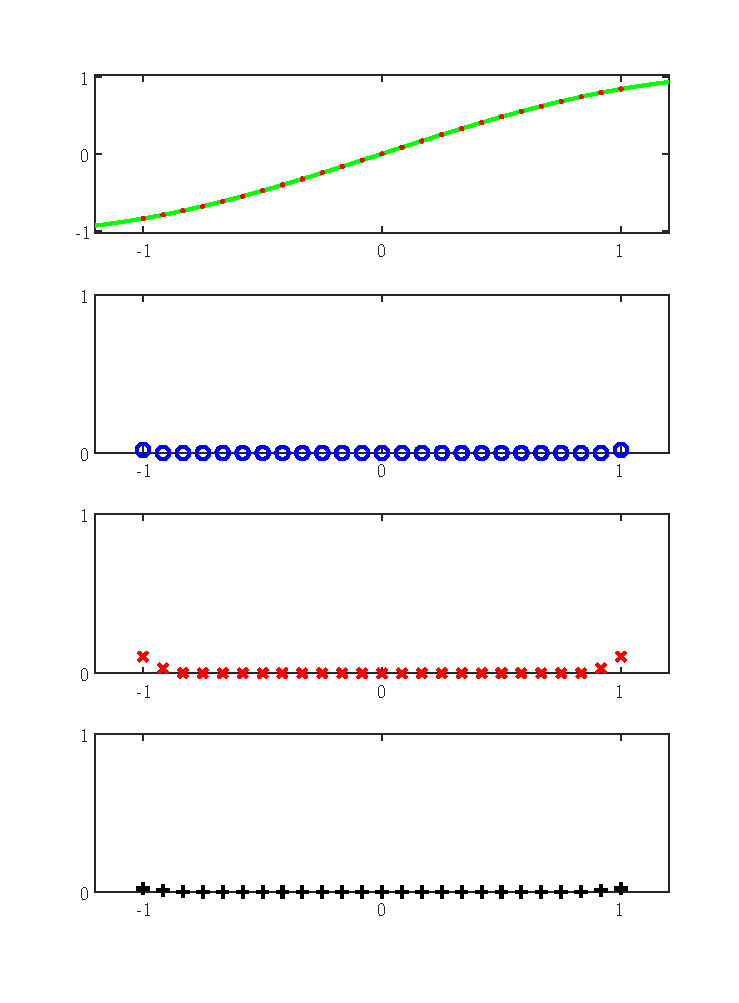
\includegraphics[width=.55\hsize]{reg_sin.pdf}
\hss
\raise 1.4cm\vbox{%
\hbox{\small$\Cal C^0$}
\kern 1.4cm
\hbox{\small$\Cal C^2$}
\kern 1.4cm
\hbox{\small$\Cal C^4$}
\vfil
}
\hss
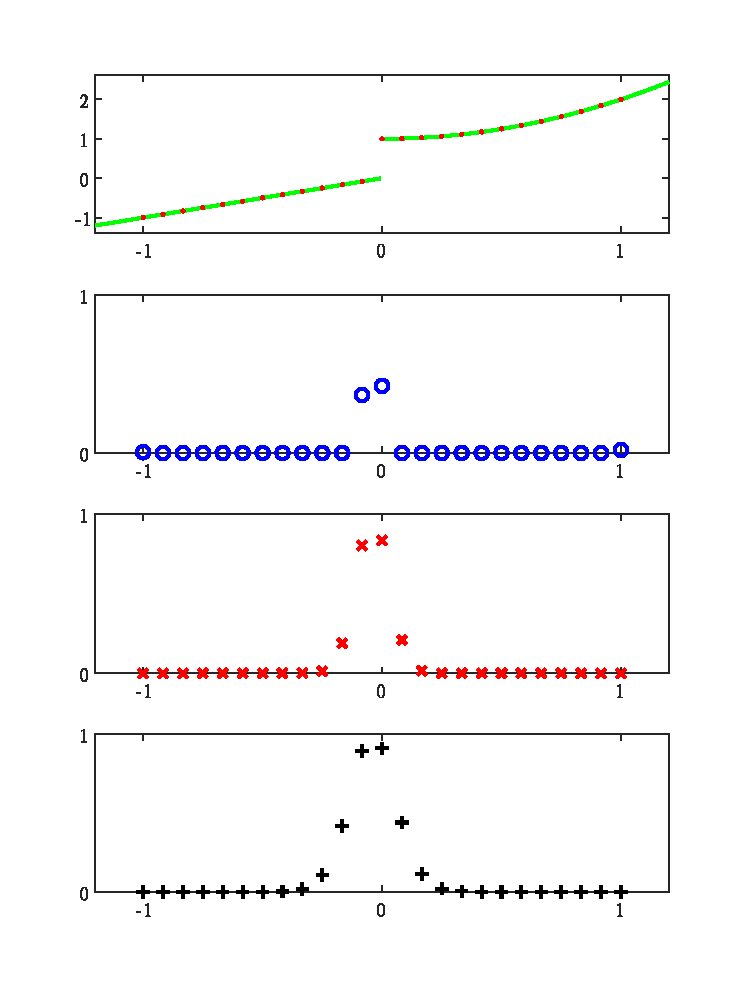
\includegraphics[width=.55\hsize]{reg_disc1.pdf}%
\kern-.7cm}
\vss
\end{frame}


\begin{frame}
\null\vskip.3cm
\line{\kern-.8cm
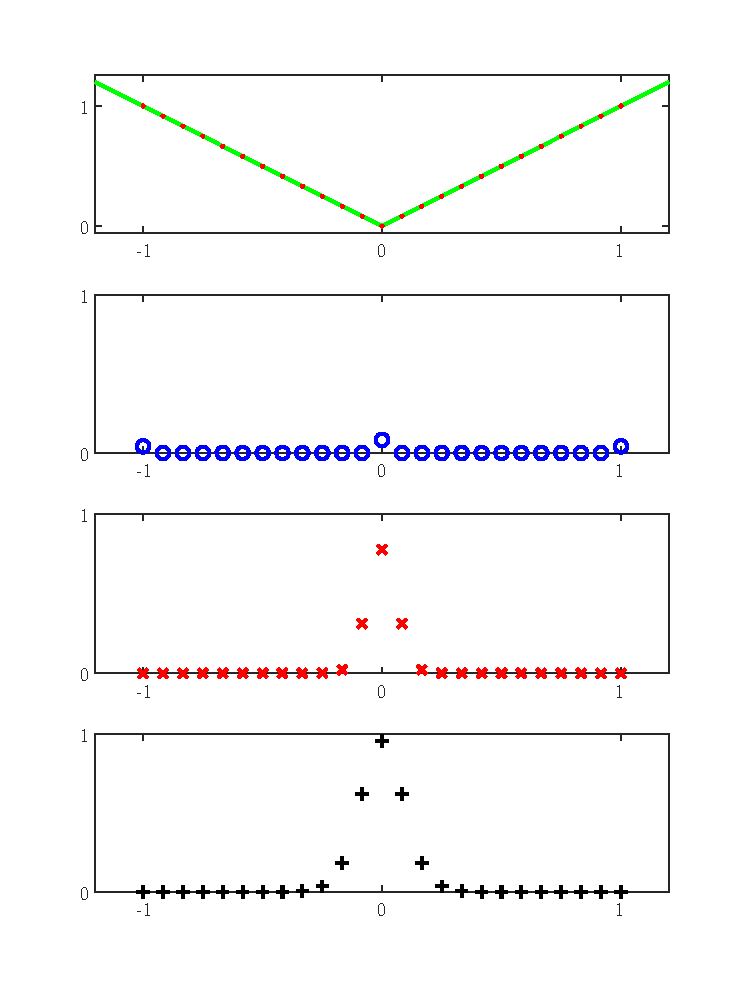
\includegraphics[width=.55\hsize]{reg_abs.pdf}
\hss
\raise 1.4cm\vbox{%
\hbox{\small$\Cal C^0$}
\kern 1.4cm
\hbox{\small$\Cal C^2$}
\kern 1.4cm
\hbox{\small$\Cal C^4$}
\vfil
}
\hss
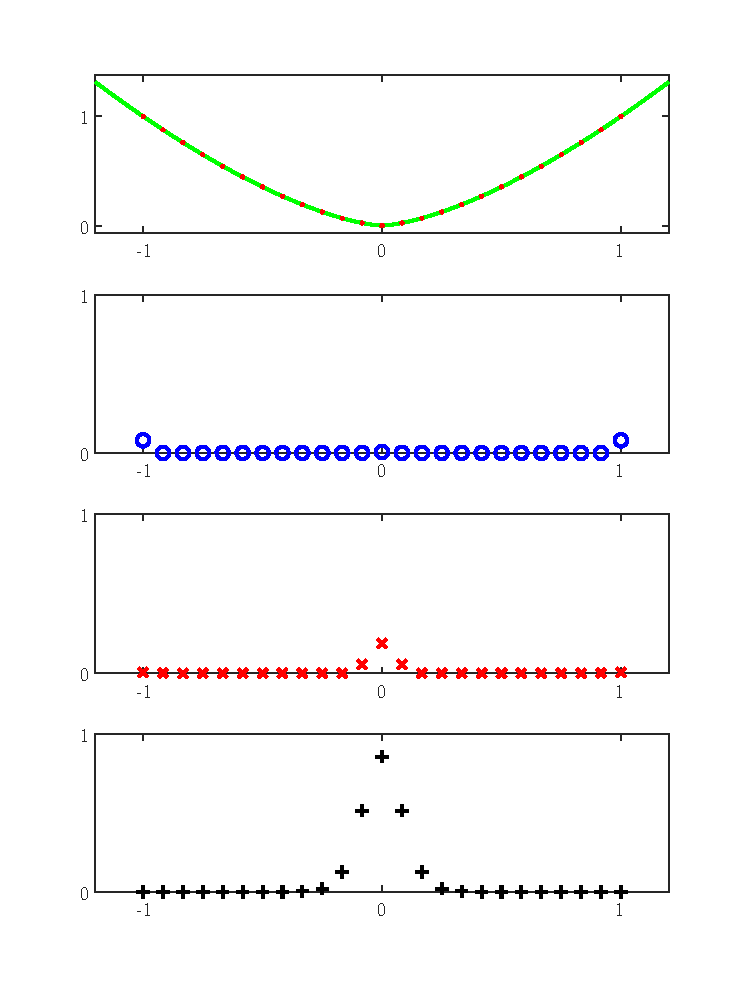
\includegraphics[width=.55\hsize]{reg_c1notc2.pdf}%
\kern-.7cm}
\vss
\end{frame}
\endcomment







\begin{frame}

\bigskip
\begin{itemize}
\item
Dal punto di vista operativo, $\widehat{\bm Q}$ si calcola come $\bar{\bm Q} = \bm Q(\bar\varepsilon)$ per un opportuno~$\bar\varepsilon$.
%Possiamo classificare la regolarità di $f$ mediante i dati $(X, F)$ utilizzando una funzione $\phi$ e una soglia $\tau>0$:

\bigskip\medskip

\item
Possiamo classificare la regolarità di un insieme di dati $(X,F)$ utilizzando una funzione~$\phi$ e una soglia~$\tau>0$:
$$
\Cal R(X, F) = \begin{cases}
				\phantom{-}1& \text{ se $\norm{\bar{\bm Q}}_1 \leq \tau$\qquad “regolare”} \\
				-1& \text{ se $\norm{\hbyw{3ex}{0em}\bar{\bm Q}}_1 > \tau$\qquad “non regolare”}. 
			   \end{cases}
$$
\end{itemize}
%La scelta di $\tau$  {\em non} dipende dai dati che si devono classificare.


\end{frame}



%\begin{frame}
%\frametitle{Esempi: scelta di $\norm{\>}_1$}
%\end{frame}




\section{Suddivisione del dominio}
\begin{frame}
\frametitle{Suddivisione del dominio}
%\alert{Problema}:  Ricostruire  fedelmente una funzione $f:\Omega\to\R$ a partire da un insieme di dati $(X, f(X))$, sapendo che $f$ è regolare su sottoinsiemi $\Omega_j$ disgiunti tali che $\Omega = \cup_j \Omega_j$, ed è discontinua lungo $\partial \Omega_j$, senza avere informazioni sui sottodomini $\Omega_j$.

%\bigskip

È possibile utilizzare $\bar{\bm Q}$ e il classificatore di regolarità $\Cal R$ per analizzare localmente in $\Omega$ i dati $(X, f(X))$ e assegnarli al loro sottodominio di appartenenza, ottenendo sottoinsiemi $X_j$ tali che $X_j\subset \Omega_j$.

\medskip

\begin{itemize} 
\item
Tramite $\Cal R$ si stabilisce se un sottoinsieme $Y \subset X$ è contenuto in un solo dominio $\Omega_j$.

\medskip

\item
Procedendo con successive analisi locali si  estende l’insieme di nodi fino ad includere tutti i punti $X_j\subset\Omega_j$.

\medskip

\item
Quando $\Cal R(Y, f(Y)) = -1$, si utilizza $\bar{\bm Q}$ per capire quali punti rimuovere, poiché  appartenenti ad un differente  sottodominio .
\end{itemize}
\end{frame}


\begin{frame}
\null\vskip.2cm
\foreach \i in {1,2,...,31}{
\only<\i>{\line{\hfil\includegraphics[width=.75\hsize]{anim_\i.pdf}\hfil}\vss}
}
\end{frame}


\begin{frame}
\def\franke{\operatorname{franke}}
%%%%%%%%%%%%%%%%%
\rlap{\vbox to 0pt{\hsize=.5\hsize \scriptsize 
							$\phi = \hbox{Wendland } \Cal C^0$, \quad $\tau = 0.2$ \\
							\vskip1ex
							$N = 2^{10}$ (Halton),\quad $\,\,\,k = 8^2$\\
							\vss}}
\line{%
\kern-1.3cm
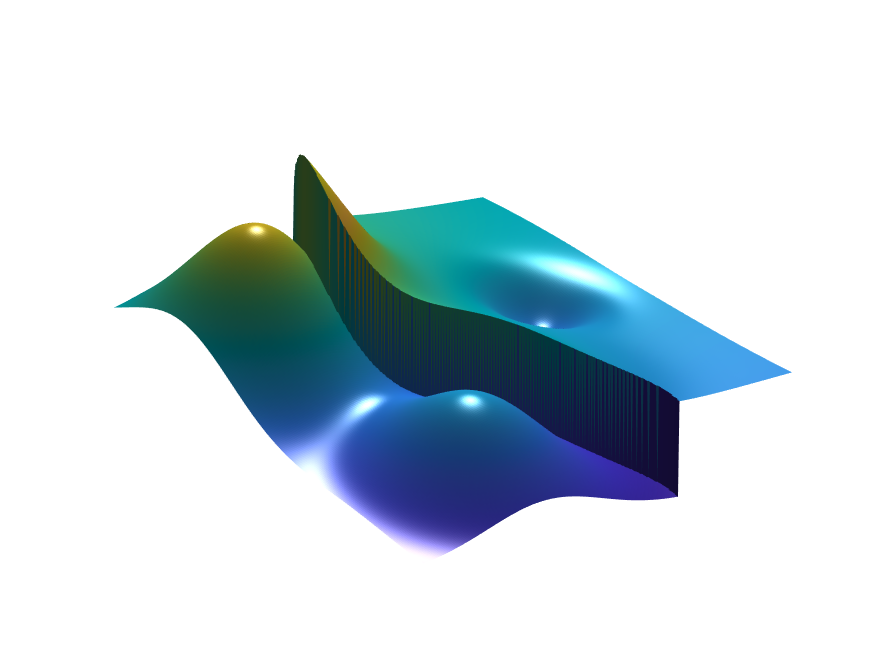
\includegraphics[width=.6\hsize]{f1_ori.pdf}
\hss
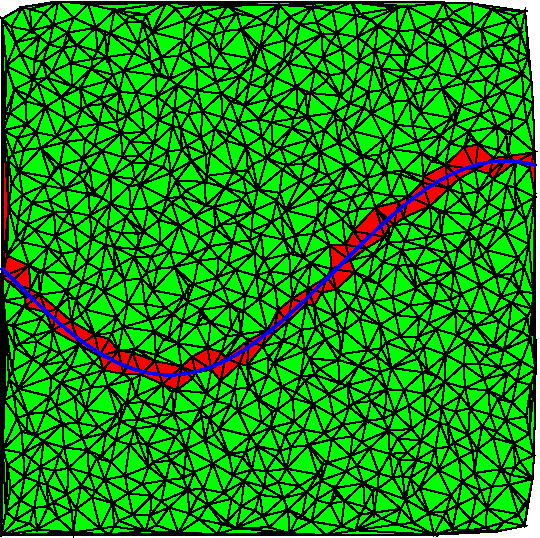
\includegraphics[width=.55\hsize]{f1.pdf}
\kern-.5cm}
\vskip.5cm
\line{\scriptsize\hfil$h_1(x,y) = \begin{cases}\franke(x,y), & \text{se $y\geq \frac12-\frac15\sin(5x)$} \\
                  \franke(x,y) - \frac12, & \text{se $y\leq \frac12-\frac15\sin(5x)$}
                  \end{cases}$\hfil}

\end{frame}


\begin{frame}
\def\franke{\operatorname{franke}}
%%%%%%%%%%%%%%%%%
\rlap{\vbox to 0pt{\hsize=.5\hsize \scriptsize 
							$\phi = \hbox{Wendland } \Cal C^0$, \quad $\tau = 0.2$ \\
							\vskip1ex
							$N = 2^{10}$ (Halton),\quad $\,\,\,k = 8^2$\\
							\vss}}
\line{%
\kern-1.3cm
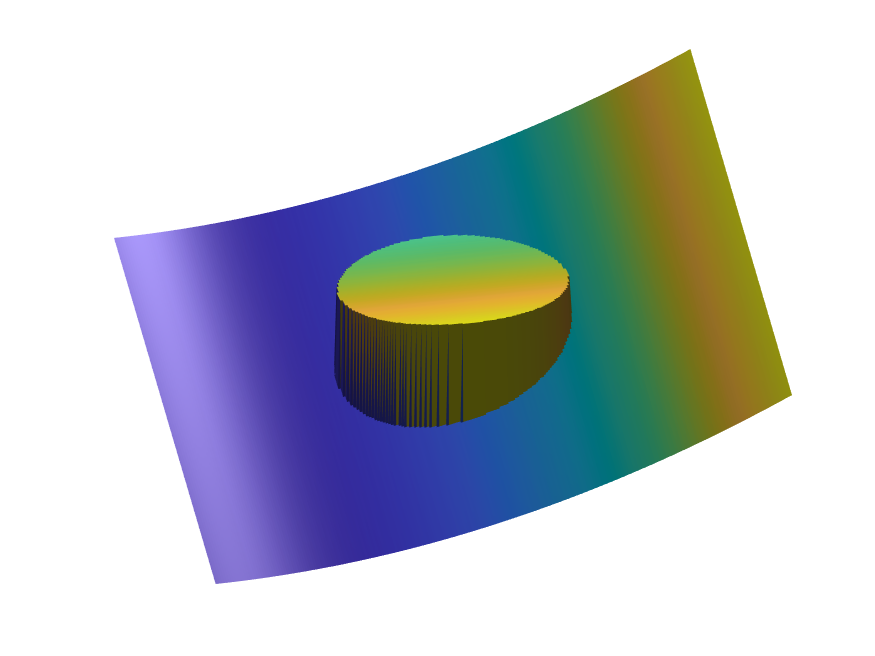
\includegraphics[width=.6\hsize]{f4_ori.pdf}
\hss
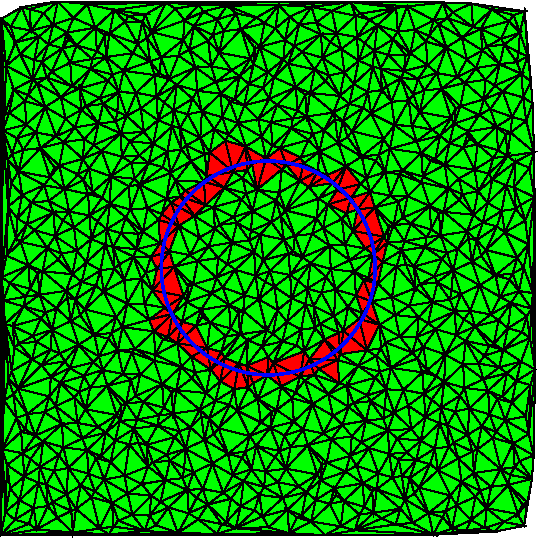
\includegraphics[width=.55\hsize]{f4.pdf}
\kern-.5cm}
\vskip.5cm
\line{\scriptsize\hfil$h_2(x,y) = \begin{cases}x^2, & \text{se $(x-\frac12)^2+(y-\frac12)^2<(\frac15)^2$} \\
                   y^2-\frac12, & \text{se $(x-\frac12)^2+(y-\frac12)^2\geq(\frac15)^2$}
                  \end{cases}$\hfil}

\end{frame}

\begin{frame}
\def\franke{\operatorname{franke}}
%%%%%%%%%%%%%%%%%
\rlap{\vbox to 0pt{\hsize=.5\hsize \scriptsize 
							$\phi = \hbox{Wendland } \Cal C^0$, \quad $\tau = 0.2$ \\
							\vskip1ex
							$N = 2^{10}$ (Halton),\quad $\,\,\,k = 8^2$\\
							\vss}}
\line{%
\kern-1.3cm
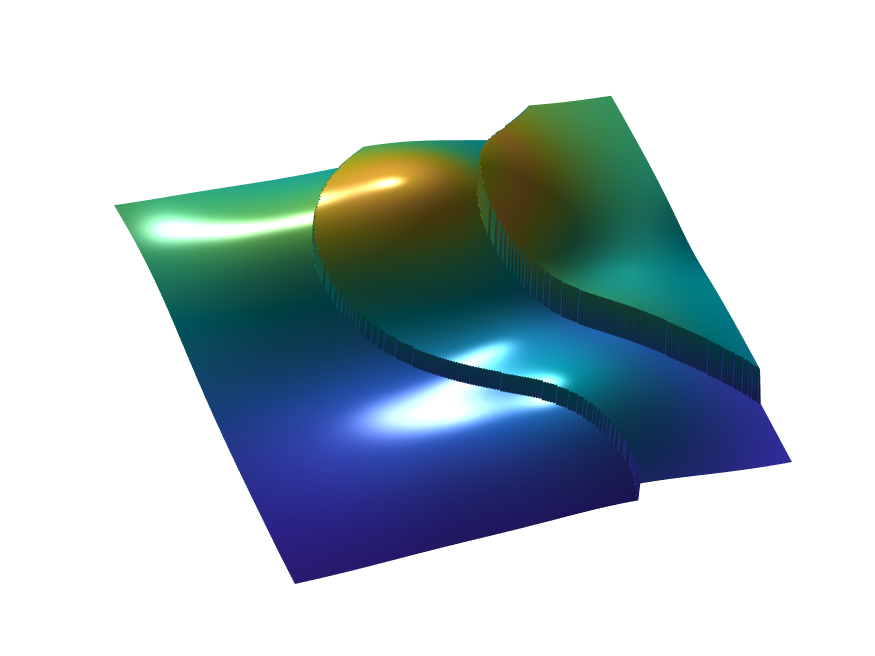
\includegraphics[width=.6\hsize]{f9_ori.pdf}
\hss
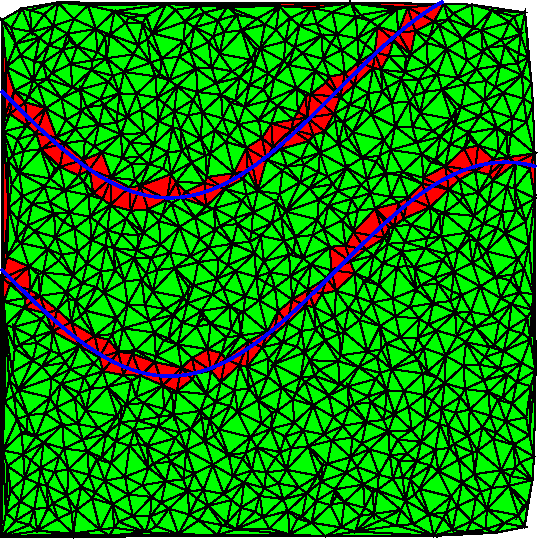
\includegraphics[width=.55\hsize]{f9.pdf}
\kern-.5cm}
\vskip.5cm
\line{\scriptsize\hfil$h_3(x,y) = h_1(x,y) + 2h_1(x, y-{\textstyle\frac13})$\hfil}

\end{frame}


\begin{frame}
\def\franke{\operatorname{franke}}
%%%%%%%%%%%%%%%%%
\rlap{\vbox to 0pt{\hsize=.5\hsize \scriptsize 
							$\phi = \hbox{Wendland } \Cal C^2$, \quad $\tau = 0.2$ \\
							\vskip1ex
							$N = 2^{10}$ (Halton),\quad $\,\,\,k = 8^2$\\
							\vss}}
\line{%
\kern-1.3cm
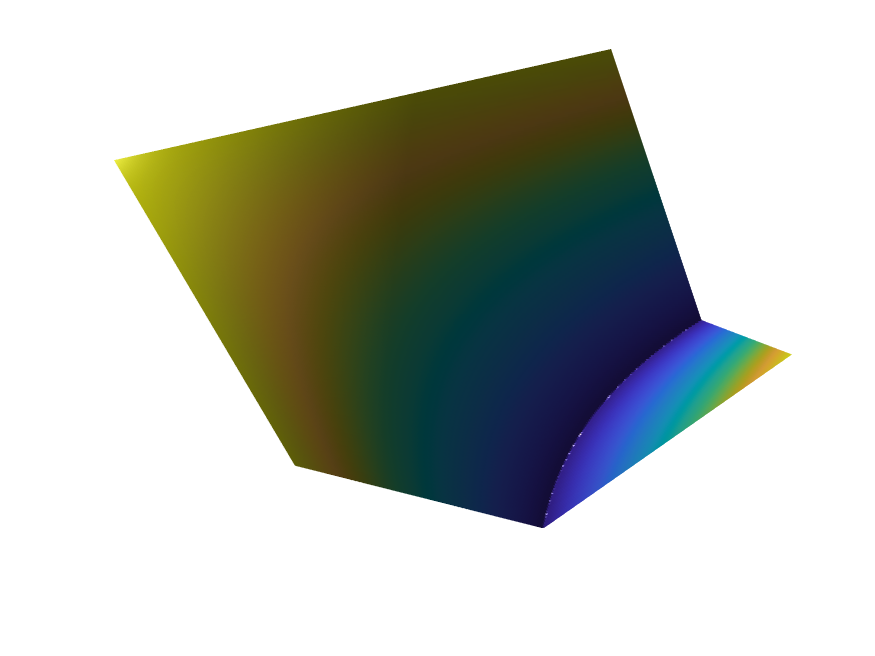
\includegraphics[width=.6\hsize]{f6_ori.pdf}
\hss
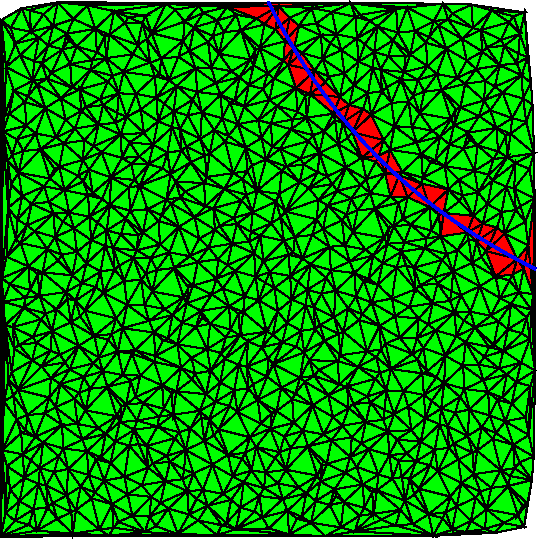
\includegraphics[width=.55\hsize]{f6.pdf}
\kern-.5cm}
\vskip.5cm
\line{\scriptsize\hfil$h_4(x,y) = \left|\frac12-xy\right|$\hfil}

\end{frame}



\section{Ricostruzione}
\begin{frame}
\frametitle{Ricostruzione}
Una volta separato $X$ in sottoinsiemi $X_j$ tali che $X_j\subset\Omega_j$ bisogna effettivamente ricostruire i sottodomini $\Omega_j$.

\bigskip

Supponendo di aver ottenuto delle ricostruzioni $\widetilde\Omega_j$ di ciascun $\Omega_j$, la ricostruzione $s$ della funzione campionata $f$ si ottiene nel seguente modo:
$$
s(y) = \begin{cases}
		s_1(y) & \text{se $y\in\widetilde\Omega_1$}\\
		s_2(y) & \text{se $y\in\widetilde\Omega_2$}\\
		\hbyw{0ex}{1em}\vdots & \hbyw{0ex}{2em}\vdots \\
		s_M(y) & \text{se $y\in\widetilde\Omega_M$}\\
            \end{cases}\qquad\text{$s_j$ interpolante di $(X_j, f(X_j))$.}
$$

\bigskip

Per ottenere $\{\widetilde\Omega_j\}_{j=1}^M$ a partire da $\{X_j\}_{j=1}^M$ utilizziamo le \alert{Support Vector Machines} (SVM). 
\end{frame}



\begin{frame}
\frametitle{Support Vector Machines}
SVM sono modelli binari.  Tuttavia si possono estendere a modelli multiclasse, che permettono di separare un numero arbitrario $M$ di insiemi di punti $\{X_j\}_{j=1}^M$.

\bigskip

Supponiamo di avere soltanto due sottoinsiemi di locazioni, $X_1$, $X_2$.
\begin{itemize}
\item Si usa una funzione~$\Theta:\R^2\to V$ (\alert{feature map}) per trasformare ciascun $X_j\subset\R^2$ in $\Theta(X_j) = \{\Theta(x):x\in X_j\}\subset V$, con $\dim V >> 2$.
\item Si determina un iperpiano in $V$ che separa $\Theta(X_1)$ da $\Theta(X_2)$, descritto implicitamente da
$$
h(x) = \langle \omega, \Theta(x) \rangle_V + b, \quad \omega, b\in V, \quad x\in\Omega
$$
\item Si ottengono infine i sottodomini $\widetilde\Omega_1$, $\widetilde\Omega_2$ nel seguente modo:
$$
\begin{aligned}
\widetilde\Omega_1 &= \{x\in \Omega : h(x) \geq 0\}\\
\widetilde\Omega_2 &= \{x\in \Omega : h(x) < 0\}
\end{aligned}
$$
\end{itemize}
\end{frame}


\begin{frame}
Per trovare $h(x) = \langle \omega, \Theta(x) \rangle_V + b$ si risolve un problema di ottimizzazione:
$$
\max_{\bm \lambda}\biggl(\sum_{i=1}^N\lambda_i - {\frac12}\sum_{i=1}^N\sum_{j=1}^N\lambda_i z_i\,\langle \Theta(x_i), \Theta(x_j)\rangle_V\, \lambda_j z_j\biggr), \quad z_k = \begin{cases}\phantom-1 & \text{se $x_k\in X_1$}\\
			-1 & \text{se $x_k\in X_2$}
\end{cases}
$$
soggetto ai vincoli
$$
\left\{\begin{aligned}&\textstyle\sum_{i=1}^N\lambda_i z_i = 0\\
                & 0\leq\lambda_i\leq C\quad\text{per ogni~$i$,}\end{aligned}\right.
$$
ottenendo $w = \sum_{j=1}^N \lambda_j z_j x_j, \qquad b =\sum_{j=1}^N\lambda_j z_j\langle \Theta(x_i), \Theta(x_j)\rangle_V\, - z_i$.


\bigskip

\alert{Nota}: Il problema dipende da $x_j\in X$ solo direttamente o tramite i prodotti scalari 
$$\langle \Theta(x_i), \Theta(x_j)\rangle_V.$$
\end{frame}


\begin{frame}
\alert{Kernel trick}: $K(x,y) = \langle \Theta(x), \Theta(y)\rangle_V$.\\\smallskip
Si basa sul \alert{teorema di Mercer}, secondo il quale ogni kernel $K:\Omega\times\Omega\to\R$ simmetrico e definito positivo si decompone in
$$
K(x,y) = \langle \Theta(x), \Theta(y)\rangle_V = \sum_{i=1}^\infty \Theta_i(x)\Theta_i(y), \quad x,y\in\Omega,
$$
con $\Theta_i$ autofunzioni dell’operatore $f\mapsto\int_\Omega f(x)K(x,y)\,dx$.

\bigskip
Il kernel più utilizzato è quello gaussiano,
$$
K(x,y) = \exp(-\delta^2\,\norm{x-y}^2),\quad x,y\in\Omega,
$$
con il quale $\dim V =\infty$.

\end{frame}




\foreach \i in {1,4,9}{
\begin{frame}
\null\vskip.1cm
\line{\kern-.5cm
\vbox{\hbox{\includegraphics[width=.45\hsize]{f\i_ori.pdf}}
\hbox{\includegraphics[width=.45\hsize]{f\i_rec.pdf}}}
\hss
\raise.3cm\hbox{\includegraphics[width=.6\hsize]{f\i_curves.pdf}}}
\end{frame}
}





\part<presentation>{Bibliography}

\begin{frame}[allowframebreaks]
\frametitle{Riferimenti bibliografici}
\footnotesize
\nocite{*}
%\bibliographystyle{amsalpha}
\bibliographystyle{unsrt}
\bibliography{biblist.bib} 
\end{frame}


\foreach \i in {6}{
\begin{frame}
\null\vskip.1cm
\line{\kern-.5cm
\vbox{\hbox{\includegraphics[width=.45\hsize]{f\i_ori.pdf}}
\hbox{\includegraphics[width=.45\hsize]{f\i_rec.pdf}}}
\hss
\raise.3cm\hbox{\includegraphics[width=.6\hsize]{f\i_curves.pdf}}}
\end{frame}
}



\end{document}
